
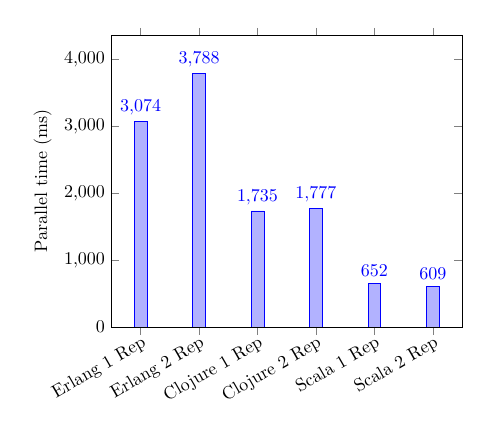
\begin{tikzpicture}[thick, scale=0.65]
  \begin{axis}[ybar,
    bar width=0.25cm,
    ymin=0,
    enlarge y limits={upper,value=0.15},
    legend style={at={(0.5,-0.25)},
    anchor=north,legend columns=-1},
    ylabel={Parallel time (ms)},
    symbolic x coords={Erlang 1 Rep, Erlang 2 Rep, Clojure 1 Rep, Clojure 2 Rep, Scala 1 Rep, Scala 2 Rep},
    xtick=data,
    xticklabel style={
        inner sep=0pt,
        anchor=north east,
        rotate=30
    },
    nodes near coords={\pgfmathprintnumber[fixed,precision=0]{\pgfplotspointmeta}},
    ]
    \addplot coordinates {(Erlang 1 Rep,3073.555556) (Erlang 2 Rep,3788.3) (Clojure 1 Rep,1734.666667) (Clojure 2 Rep,1777.333333) (Scala 1 Rep,651.8888889) (Scala 2 Rep,609.125)};
  \end{axis}
\end{tikzpicture}